\documentclass[10pt]{article}
\usepackage[letterpaper,margin=0.8in]{geometry}
\usepackage{amsmath,amssymb,amsthm}
\usepackage{graphicx}
\usepackage{microtype}
\usepackage{enumitem}
\usepackage[hidelinks]{hyperref}
\usepackage[font=small,labelfont=bf,skip=4pt]{caption}
\usepackage{booktabs}
\graphicspath{{../artifacts/}}
\setlist[itemize]{leftmargin=1.2em,itemsep=1pt,topsep=2pt}
\newtheorem{proposition}{Proposition}
\newtheorem{corollary}{Corollary}

\title{An analytic model of epistemic collapse}
\author{Helivan \quad Calcifer Computing}
\date{working note}

\begin{document}
\maketitle

\paragraph{Summary.}
Because agents relay verbatim and an LLM's answering behavior is a measured multinomial over a small set of context states, the probability of epistemic collapse can be computed rather than simulated. We derive (i) the probability that a single agent can answer a question, from a renewal argument on its memory; (ii) the probability that a question is in collapse, from a birth--death chain over how many agents hold it; and (iii) the probability of $\chi$-epistemic collapse, from a binomial count over questions. The model has no fitted parameters and reproduces simulation for three strategies --- no mitigation, sharing secondhand information, and books --- across two decades of environment size (Fig.~\ref{fig:analytic}). To leading order it yields a closed-form law for the \emph{epistemic capacity} $M^\star(\chi)$ --- the largest environment a system can sustain with less than a proportion $\chi$ of its questions in collapse --- and for the \emph{epistemic efficiency} of each mitigation, $\Gamma(\chi) = M^\star_{\text{strategy}}(\chi)/M^\star_{\text{none}}(\chi)$: sharing secondhand information raises capacity by a factor $x/(1-e^{-x})$ with $x = K\ln(1/\chi)/(NE)$ --- about $10$--$20\%$ here --- while books raise it by $\approx (1-p_w)(1 + fKb/E)$ --- about $3.5\times$ here (Sec.~\ref{sec:prevention}).

\section{Model and notation}
$N$ agents; an environment of $M$ questions; each agent spends $B$ actions per step, of which a fraction $\alpha$ query the environment ($E = \alpha B$ per step, questions drawn uniformly) and $K = (1-\alpha)B$ ask peers. Asks target questions the asker cannot currently answer. Memory is unbounded; retrieval keeps the $k$ entries with the largest $\langle q,k\rangle e^{-c\,\Delta t}$. An exact-match entry scores $1$ at insertion, any other entry scores at most $\sigma<1$, so an entry received $a$ steps ago is outscored by a newer entry only after $\Delta = \ln(1/\sigma)/c$ steps. Write $D = \lfloor \Delta \rfloor$.

\paragraph{Retention.} An entry for $q$ inserted $a$ steps ago is retrievable iff $a \le D$, or fewer than $k$ new entries have been inserted in the $a - D$ steps since. Each of the $B$ actions inserts an entry with probability $q_{\mathrm{ins}}$ (an observation always inserts; an ask inserts iff it is answered), so the count over $m$ steps is $\mathrm{Bin}(mB, q_{\mathrm{ins}})$. Forgetting is therefore \emph{activity-dependent}: the busier the agent, the faster old entries are crowded out.

\paragraph{Gate.} Given its context, an agent answers or abstains. For the LLM we measured $P(\text{IDK} \mid q \text{ in context}) = \varepsilon$ ($\approx 0.03$--$0.05$) and $P(\text{answer} \mid q \text{ not in context}) \approx 0$; the toy has $\varepsilon = 0$.

\section{Results}

\begin{proposition}[Single agent]
Let $\mu = 1 - (1-\alpha/M)^B$ be the per-step probability that an agent observes $q$. With observation as the only way to (re)acquire $q$, the stationary probability that the agent cannot answer $q$ is
\begin{equation}
p \;=\; \sum_{a > D} \mu(1-\mu)^a \; \Pr\!\big[\mathrm{Bin}\big((a-D)B,\, q_{\mathrm{ins}}\big) \ge k\big],
\qquad q_{\mathrm{ins}} = \alpha + (1-\alpha)(1-p),
\label{eq:renewal}
\end{equation}
solved as a fixed point (asks are answered when the peer holds the question).
\end{proposition}
\noindent The age of the agent's last acquisition is geometric; the sum integrates the retention rule over that age.

\begin{proposition}[Question-level collapse]
Let $n$ be the number of agents that can answer $q$. Holders lose $q$ at rate $\delta = \mu p/(1-p)$ each (the exponential rate reproducing Eq.~\ref{eq:renewal}); each non-holder acquires it at rate $g(n)$. The stationary law of the birth--death chain is
\begin{equation}
\pi_n \;\propto\; \prod_{j=1}^{n} \frac{(N-j+1)\,g(j-1)}{j\,\delta},
\end{equation}
and the question is in epistemic collapse with probability $\pi_0^{\varepsilon} = \sum_n \pi_n \varepsilon^n$ (every holder also abstains), which is $\pi_0$ for a deterministic gate.
\end{proposition}
\noindent The strategies differ only in the acquisition rate:
\begin{itemize}
  \item \textbf{No mitigation.} $g(n) = \mu$: agents are independent, $\pi_0 = p^N$.
  \item \textbf{Sharing secondhand information.} $g(n) = \mu + \frac{K}{Mp}\frac{n}{N-1}$: an agent spends its $K$ asks on its $\approx Mp$ unknown questions and succeeds iff the random peer holds $q$. Answered asks also insert, so $q_{\mathrm{ins}} = \alpha + (1-\alpha)\,\Pr[\text{peer holds } q \mid \text{asker lacks } q]$ from the chain.
  \item \textbf{Books.} $g(n) = \mu' + \frac{fK'}{Mp}\,b$, where a fraction $f$ of asks read the book, $b$ is the fraction of questions the book covers, and a write tax $p_w$ scales the budget ($\mu' , K' \leftarrow (1-p_w)\mu, (1-p_w)K$). The book never forgets; it gains an uncovered question when a committing writer holds it, and commits arrive at rate $N p_w/W$, so
  \begin{equation}
  \frac{d(1-b)}{dt} = -\frac{N p_w}{W}\,\big(1 - p_u(b)\big)\,(1-b),
  \end{equation}
  with $p_u(b)$ from Eq.~\ref{eq:renewal} with the reads' extra insertions. Agents are again independent given $b$.
\end{itemize}

\begin{proposition}[System-level collapse]
Treating questions as independent, the number in collapse is $\mathrm{Bin}(M, \pi_0)$ and
\begin{equation}
\Pr[\chi\text{-epistemic collapse}] \;=\; \Pr\big[\mathrm{Bin}(M, \pi_0) \ge \lceil \chi M \rceil\big].
\end{equation}
\end{proposition}
\noindent Since the binomial concentrates, this is nearly a step function at $\pi_0 = \chi$: $\chi$-collapse is a sharp transition in the environment size.

\begin{corollary}[Epistemic capacity, no mitigation]
For $M \gg B$, $1-p \approx E\tau/M$ with $\tau \approx D + 1 + k/(Bq_{\mathrm{ins}})$ the mean retention time, so $\pi_0 = p^N \approx e^{-NE\tau/M}$ and the system enters $\chi$-collapse at
\begin{equation}
M^\star \;\approx\; \frac{N\,E\,\tau}{\ln(1/\chi)} .
\end{equation}
\end{corollary}
\noindent The system survives while its \emph{collective observational memory} --- agents $\times$ observations per step $\times$ steps each observation is retained --- exceeds the environment size by a factor $\ln(1/\chi)$. Memory decay enters only through $\tau$; environment speed does not enter at all, which is why speed moves staleness but not collapse.

\section{Validation}
Figure~\ref{fig:analytic} compares the model with the simulator ($N=10$, $B=11$, $E=3$, $k=3$, $\sigma=0.5$, $16$ seeds, steady state over the final $200$ of $600$ steps). No parameter is fitted. Across all three strategies, both decay rates and nine environment sizes, the per-question collapse probability matches to within $0.03$, and the location of the $\chi$-collapse transition matches; the one visible miss is mimesis at $c=0.5$, $M=50$, which sits on the steep part of the transition. The book coverage $b(t)$ is predicted to within $0.02$. Table~\ref{tab:mstar} compares the closed-form $M^\star$ with the exact solution; it is within $4\%$ for slow decay and overestimates by $\approx 25\%$ for fast decay, where retention lasts only two to three steps and the discreteness of time matters.

\begin{figure}[h]
  \centering
  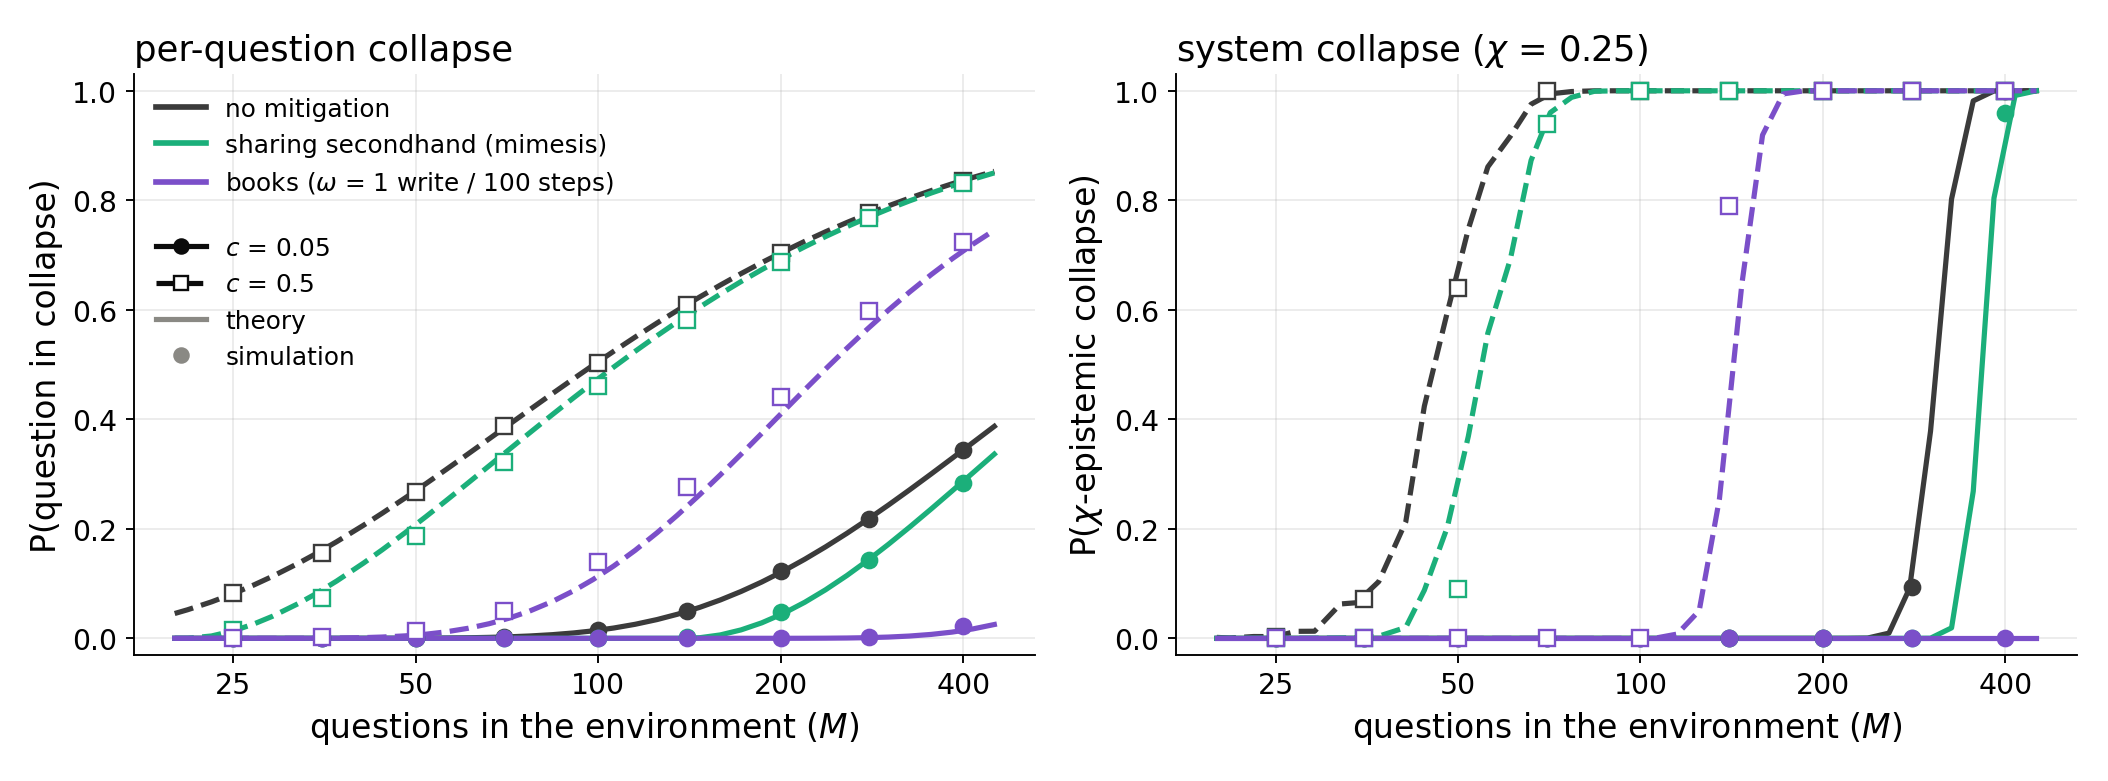
\includegraphics[width=\textwidth]{fig_analytic_collapse.png}
  \caption{\textbf{Theory (lines) vs.\ simulation (markers), no fitted parameters.} Left: probability that a question is in epistemic collapse. Right: probability of $\chi$-epistemic collapse, $\chi=0.25$. Books: one completed write per agent per 100 steps ($p_w=0.05$, $W=5$), all asks read the book.}
  \label{fig:analytic}
\end{figure}

\begin{table}[h]
\centering
\small
\begin{tabular}{cccc}
\toprule
$c$ & $\chi$ & $M^\star$ exact & $N E \tau / \ln(1/\chi)$ \\
\midrule
0.05 & 0.25 & 307 & 319 \\
0.05 & 0.50 & 618 & 643 \\
0.5  & 0.25 & 47  & 59 \\
0.5  & 0.50 & 98  & 123 \\
\bottomrule
\end{tabular}
\caption{Epistemic capacity: exact solution of the model vs.\ the closed form.}
\label{tab:mstar}
\end{table}

\section{How much do mitigations prevent collapse?}
\label{sec:prevention}
In the collapse regime (holders of a question are rare, $M \gg B$) every strategy acts in the same way: it multiplies the system's collective observational memory $N E \tau$ by an amplification factor $\Gamma \ge 1$ (or $<1$ if it hurts). Consequently
\begin{equation}
\pi_0^{\text{strategy}} \;\approx\; \big(\pi_0^{\text{none}}\big)^{\Gamma},
\qquad
M^\star_{\text{strategy}} \;\approx\; \Gamma\, M^\star_{\text{none}} ,
\label{eq:gamma}
\end{equation}
so $\Gamma$ is the \emph{epistemic efficiency}: the multiple by which a strategy enlarges the environment the system can track before collapsing.

\begin{proposition}[Sharing secondhand information]
With per-holder transmission rate $a \approx K/M$ (asks from the $N-1$ non-holders, answered by one holder), loss rate $1/\tau$ and immigration $N\mu \approx NE/M$ from observation, the number of holders is a branching process with immigration and reproduction number $R = K\tau/M$. Its stationary law is negative binomial, with
\begin{equation}
\pi_0^{\text{mim}} = (1-R)^{N E \tau/(M R)}
\;=\; \exp\!\Big(-\frac{N E \tau}{M}\,\varphi(R)\Big),\qquad \varphi(R) = \frac{-\ln(1-R)}{R},
\end{equation}
so $\Gamma_{\text{mim}} = \varphi(R) \cdot \tau_{\text{mim}}/\tau$. At the collapse threshold $R$ is itself fixed by $M^\star$, and solving gives a law that does not involve memory decay at all:
\begin{equation}
\Gamma^\star_{\text{mim}} \;=\; \frac{x}{1 - e^{-x}}, \qquad x = \frac{K \ln(1/\chi)}{N E}.
\end{equation}
\end{proposition}
\noindent Mimesis is therefore strong only when $x \gtrsim 1$: when an agent's ask bandwidth $K$ is large compared with the \emph{population's} total observation rate $NE$. It can only amplify evidence that someone has observed, and near the threshold a question is observed so rarely that its few holders forget it before peers ask. In our setting $x = 0.37$ ($\chi = 0.25$) and $0.18$ ($\chi = 0.5$): mimesis enlarges the trackable environment by only $20\%$ and $10\%$. The benefit shrinks as the population or its observation rate grows, and as the collapse proportion becomes stricter.

\begin{proposition}[Books]
Agents are independent given book coverage $b(t)$, and a read of a covered question acquires it exactly as an observation does. Hence books add $fK'b$ to the per-agent source rate, at the cost of the write tax and of extra crowding:
\begin{equation}
\Gamma_{\text{books}}(t) \;=\; (1 - p_w)\,\frac{\tau_b}{\tau}\,\Big(1 + \frac{f K\, b(t)}{E}\Big)
\;\xrightarrow{\;t\to\infty\;}\; (1 - p_w)\,\frac{\tau_b}{\tau}\,\frac{E + fK}{E},
\end{equation}
with $b(t)$ from the coverage equation and $\tau_b$ the retention time under the heavier insertion load of reading.
\end{proposition}
\noindent A book turns the peer-ask budget into source bandwidth: with every ask reading the book ($f=1$) the steady-state factor is $\approx (1-p_w)\,\tau_b/(\tau\,\alpha)$ --- the inverse of the fraction of the budget spent observing. In our setting $\Gamma_{\text{books}} \approx 3.5$. The write rate $\omega = p_w/W$ controls only how fast $\Gamma$ is reached, through $b(t)$; the write probability $p_w$ additionally taxes the steady state.

\begin{table}[h]
\centering\small
\begin{tabular}{llcccc}
\toprule
& & \multicolumn{2}{c}{$\chi = 0.25$} & \multicolumn{2}{c}{$\chi = 0.5$}\\
strategy & $c$ & exact & closed form & exact & closed form \\
\midrule
mimesis & 0.05 & 1.19 & 1.23 & 1.09 & 1.10 \\
mimesis & 0.5  & 1.19 & 1.22 & 1.09 & 1.10 \\
books ($b=1$) & 0.05 & 3.62 & 3.48 & 3.51 & 3.48 \\
books ($b=1$) & 0.5  & 3.39 & 3.48 & 3.15 & 3.48 \\
\bottomrule
\end{tabular}
\caption{Epistemic efficiency $\Gamma = M^\star_{\text{strategy}}/M^\star_{\text{none}}$: exact solution of the chain model vs.\ closed form. Books: $p_w = 0.05$, $f = 1$, full coverage.}
\label{tab:gamma}
\end{table}

\begin{figure}[h]
  \centering
  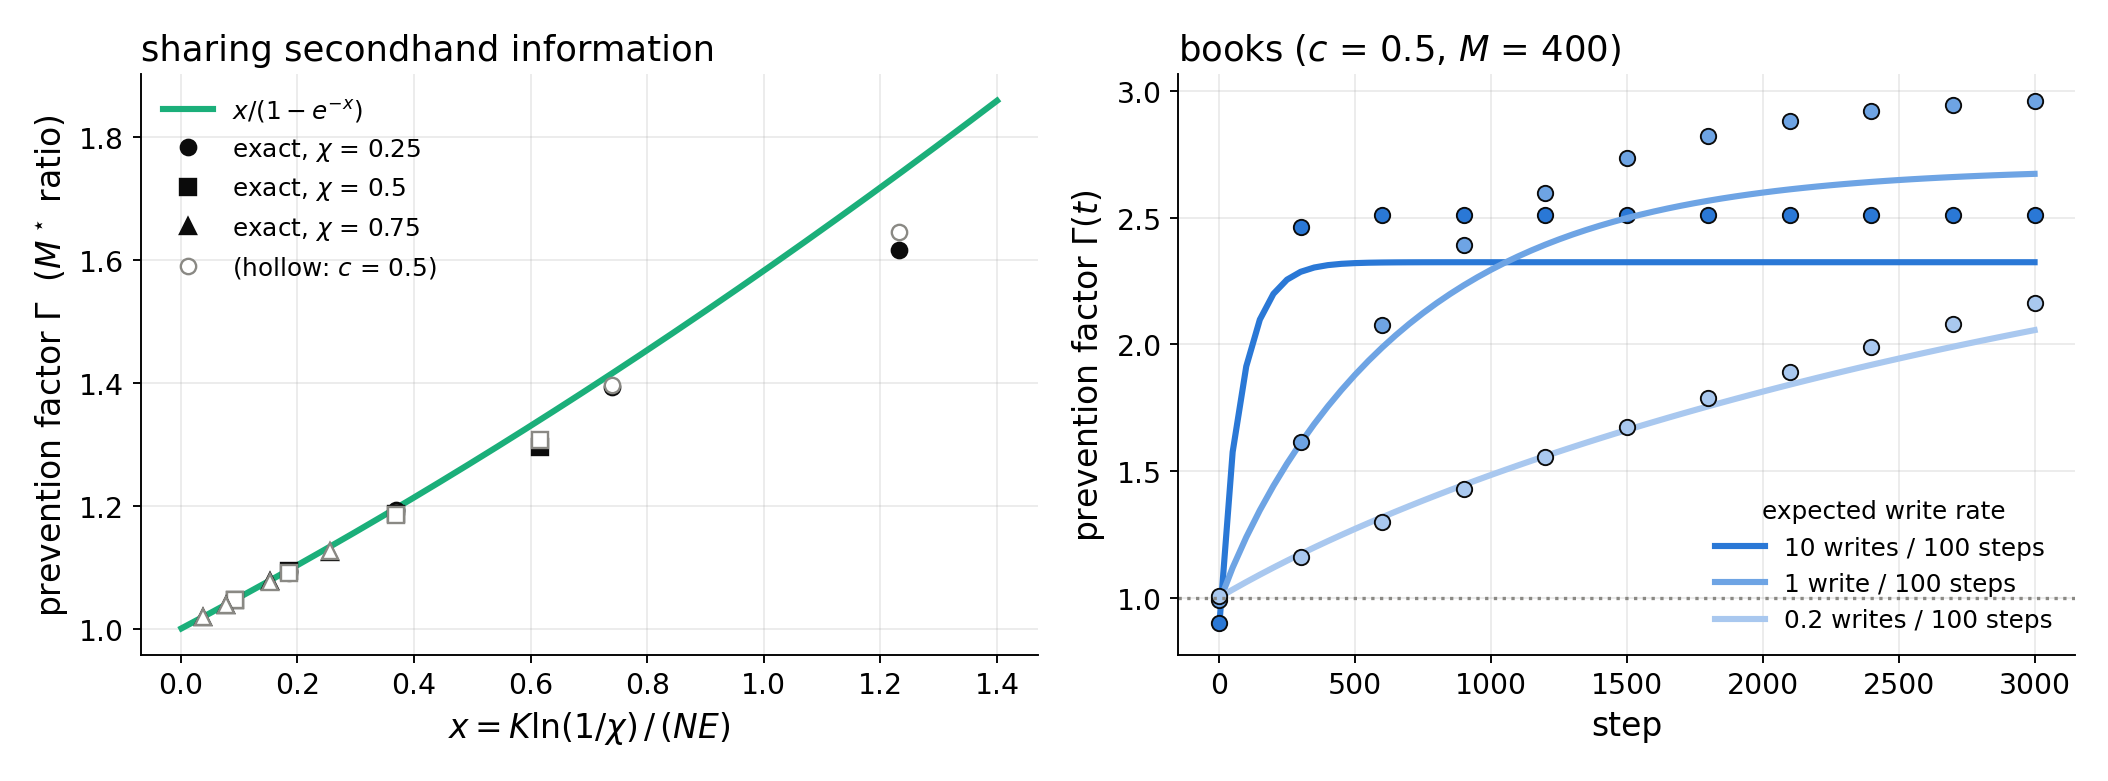
\includegraphics[width=\textwidth]{fig_prevention.png}
  \caption{\textbf{Epistemic efficiency.} Left: mimesis at the collapse threshold collapses onto the one-parameter curve $x/(1-e^{-x})$ across population sizes, decay rates and collapse proportions (markers: exact model). Right: books over time for three write rates at $c=0.5$, $M=400$; the book's value accumulates as it fills in (lines: closed form; markers: exact model). The closed form is exact while the book fills and underestimates the plateau by $\approx 8$--$10\%$ once coverage is complete, when holders are no longer rare.}
  \label{fig:prevention}
\end{figure}

The closed forms are rare-holder limits: they are most accurate near the collapse threshold, which is where they are needed, and conservative (they slightly underestimate efficiency) when agents hold a substantial share of the environment. Against simulation, $\pi_0^{\text{none}}$ raised to $\Gamma$ predicts the collapsed fraction under mimesis to within $0.03$ and under books to within $0.03$ once the crowding ratio $\tau_b/\tau$ is included.

\paragraph{Caveats.} (1) Questions are treated as independent; they are coupled weakly through shared insertion rates. (2) Losses are modeled at a constant rate chosen to reproduce the exact single-agent occupancy; the true loss hazard has a safe period of $D$ steps. (3) Asks are assumed spread over unknown questions and capped by nothing; this overpredicts mimesis at small $M$ (agent-level abstention), not collapse. (4) The book result assumes that reading the book re-grounds a forgotten fact even when the agent once held newer, now crowded-out evidence (\texttt{book\_reground=True}); the simulator's default does not, which the model reproduces only with that flag.

\end{document}
